% Options for packages loaded elsewhere
% Options for packages loaded elsewhere
\PassOptionsToPackage{unicode}{hyperref}
\PassOptionsToPackage{hyphens}{url}
\PassOptionsToPackage{dvipsnames,svgnames,x11names}{xcolor}
%
\documentclass[
  titlepage]{article}
\usepackage{xcolor}
\usepackage{amsmath,amssymb}
\setcounter{secnumdepth}{5}
\usepackage{iftex}
\ifPDFTeX
  \usepackage[T1]{fontenc}
  \usepackage[utf8]{inputenc}
  \usepackage{textcomp} % provide euro and other symbols
\else % if luatex or xetex
  \usepackage{unicode-math} % this also loads fontspec
  \defaultfontfeatures{Scale=MatchLowercase}
  \defaultfontfeatures[\rmfamily]{Ligatures=TeX,Scale=1}
\fi
\usepackage{lmodern}
\ifPDFTeX\else
  % xetex/luatex font selection
\fi
% Use upquote if available, for straight quotes in verbatim environments
\IfFileExists{upquote.sty}{\usepackage{upquote}}{}
\IfFileExists{microtype.sty}{% use microtype if available
  \usepackage[]{microtype}
  \UseMicrotypeSet[protrusion]{basicmath} % disable protrusion for tt fonts
}{}
\makeatletter
\@ifundefined{KOMAClassName}{% if non-KOMA class
  \IfFileExists{parskip.sty}{%
    \usepackage{parskip}
  }{% else
    \setlength{\parindent}{0pt}
    \setlength{\parskip}{6pt plus 2pt minus 1pt}}
}{% if KOMA class
  \KOMAoptions{parskip=half}}
\makeatother
% Make \paragraph and \subparagraph free-standing
\makeatletter
\ifx\paragraph\undefined\else
  \let\oldparagraph\paragraph
  \renewcommand{\paragraph}{
    \@ifstar
      \xxxParagraphStar
      \xxxParagraphNoStar
  }
  \newcommand{\xxxParagraphStar}[1]{\oldparagraph*{#1}\mbox{}}
  \newcommand{\xxxParagraphNoStar}[1]{\oldparagraph{#1}\mbox{}}
\fi
\ifx\subparagraph\undefined\else
  \let\oldsubparagraph\subparagraph
  \renewcommand{\subparagraph}{
    \@ifstar
      \xxxSubParagraphStar
      \xxxSubParagraphNoStar
  }
  \newcommand{\xxxSubParagraphStar}[1]{\oldsubparagraph*{#1}\mbox{}}
  \newcommand{\xxxSubParagraphNoStar}[1]{\oldsubparagraph{#1}\mbox{}}
\fi
\makeatother

\usepackage{color}
\usepackage{fancyvrb}
\newcommand{\VerbBar}{|}
\newcommand{\VERB}{\Verb[commandchars=\\\{\}]}
\DefineVerbatimEnvironment{Highlighting}{Verbatim}{commandchars=\\\{\}}
% Add ',fontsize=\small' for more characters per line
\usepackage{framed}
\definecolor{shadecolor}{RGB}{241,243,245}
\newenvironment{Shaded}{\begin{snugshade}}{\end{snugshade}}
\newcommand{\AlertTok}[1]{\textcolor[rgb]{0.68,0.00,0.00}{#1}}
\newcommand{\AnnotationTok}[1]{\textcolor[rgb]{0.37,0.37,0.37}{#1}}
\newcommand{\AttributeTok}[1]{\textcolor[rgb]{0.40,0.45,0.13}{#1}}
\newcommand{\BaseNTok}[1]{\textcolor[rgb]{0.68,0.00,0.00}{#1}}
\newcommand{\BuiltInTok}[1]{\textcolor[rgb]{0.00,0.23,0.31}{#1}}
\newcommand{\CharTok}[1]{\textcolor[rgb]{0.13,0.47,0.30}{#1}}
\newcommand{\CommentTok}[1]{\textcolor[rgb]{0.37,0.37,0.37}{#1}}
\newcommand{\CommentVarTok}[1]{\textcolor[rgb]{0.37,0.37,0.37}{\textit{#1}}}
\newcommand{\ConstantTok}[1]{\textcolor[rgb]{0.56,0.35,0.01}{#1}}
\newcommand{\ControlFlowTok}[1]{\textcolor[rgb]{0.00,0.23,0.31}{\textbf{#1}}}
\newcommand{\DataTypeTok}[1]{\textcolor[rgb]{0.68,0.00,0.00}{#1}}
\newcommand{\DecValTok}[1]{\textcolor[rgb]{0.68,0.00,0.00}{#1}}
\newcommand{\DocumentationTok}[1]{\textcolor[rgb]{0.37,0.37,0.37}{\textit{#1}}}
\newcommand{\ErrorTok}[1]{\textcolor[rgb]{0.68,0.00,0.00}{#1}}
\newcommand{\ExtensionTok}[1]{\textcolor[rgb]{0.00,0.23,0.31}{#1}}
\newcommand{\FloatTok}[1]{\textcolor[rgb]{0.68,0.00,0.00}{#1}}
\newcommand{\FunctionTok}[1]{\textcolor[rgb]{0.28,0.35,0.67}{#1}}
\newcommand{\ImportTok}[1]{\textcolor[rgb]{0.00,0.46,0.62}{#1}}
\newcommand{\InformationTok}[1]{\textcolor[rgb]{0.37,0.37,0.37}{#1}}
\newcommand{\KeywordTok}[1]{\textcolor[rgb]{0.00,0.23,0.31}{\textbf{#1}}}
\newcommand{\NormalTok}[1]{\textcolor[rgb]{0.00,0.23,0.31}{#1}}
\newcommand{\OperatorTok}[1]{\textcolor[rgb]{0.37,0.37,0.37}{#1}}
\newcommand{\OtherTok}[1]{\textcolor[rgb]{0.00,0.23,0.31}{#1}}
\newcommand{\PreprocessorTok}[1]{\textcolor[rgb]{0.68,0.00,0.00}{#1}}
\newcommand{\RegionMarkerTok}[1]{\textcolor[rgb]{0.00,0.23,0.31}{#1}}
\newcommand{\SpecialCharTok}[1]{\textcolor[rgb]{0.37,0.37,0.37}{#1}}
\newcommand{\SpecialStringTok}[1]{\textcolor[rgb]{0.13,0.47,0.30}{#1}}
\newcommand{\StringTok}[1]{\textcolor[rgb]{0.13,0.47,0.30}{#1}}
\newcommand{\VariableTok}[1]{\textcolor[rgb]{0.07,0.07,0.07}{#1}}
\newcommand{\VerbatimStringTok}[1]{\textcolor[rgb]{0.13,0.47,0.30}{#1}}
\newcommand{\WarningTok}[1]{\textcolor[rgb]{0.37,0.37,0.37}{\textit{#1}}}

\usepackage{longtable,booktabs,array}
\usepackage{calc} % for calculating minipage widths
% Correct order of tables after \paragraph or \subparagraph
\usepackage{etoolbox}
\makeatletter
\patchcmd\longtable{\par}{\if@noskipsec\mbox{}\fi\par}{}{}
\makeatother
% Allow footnotes in longtable head/foot
\IfFileExists{footnotehyper.sty}{\usepackage{footnotehyper}}{\usepackage{footnote}}
\makesavenoteenv{longtable}
\usepackage{graphicx}
\makeatletter
\newsavebox\pandoc@box
\newcommand*\pandocbounded[1]{% scales image to fit in text height/width
  \sbox\pandoc@box{#1}%
  \Gscale@div\@tempa{\textheight}{\dimexpr\ht\pandoc@box+\dp\pandoc@box\relax}%
  \Gscale@div\@tempb{\linewidth}{\wd\pandoc@box}%
  \ifdim\@tempb\p@<\@tempa\p@\let\@tempa\@tempb\fi% select the smaller of both
  \ifdim\@tempa\p@<\p@\scalebox{\@tempa}{\usebox\pandoc@box}%
  \else\usebox{\pandoc@box}%
  \fi%
}
% Set default figure placement to htbp
\def\fps@figure{htbp}
\makeatother





\setlength{\emergencystretch}{3em} % prevent overfull lines

\providecommand{\tightlist}{%
  \setlength{\itemsep}{0pt}\setlength{\parskip}{0pt}}



 


\usepackage{fvextra}
\DefineVerbatimEnvironment{Highlighting}{Verbatim}{breaklines,commandchars=\\\{\}}
\DefineVerbatimEnvironment{OutputCode}{Verbatim}{breaklines,commandchars=\\\{\}}
\makeatletter
\@ifpackageloaded{caption}{}{\usepackage{caption}}
\AtBeginDocument{%
\ifdefined\contentsname
  \renewcommand*\contentsname{Table of contents}
\else
  \newcommand\contentsname{Table of contents}
\fi
\ifdefined\listfigurename
  \renewcommand*\listfigurename{List of Figures}
\else
  \newcommand\listfigurename{List of Figures}
\fi
\ifdefined\listtablename
  \renewcommand*\listtablename{List of Tables}
\else
  \newcommand\listtablename{List of Tables}
\fi
\ifdefined\figurename
  \renewcommand*\figurename{Figure}
\else
  \newcommand\figurename{Figure}
\fi
\ifdefined\tablename
  \renewcommand*\tablename{Table}
\else
  \newcommand\tablename{Table}
\fi
}
\@ifpackageloaded{float}{}{\usepackage{float}}
\floatstyle{ruled}
\@ifundefined{c@chapter}{\newfloat{codelisting}{h}{lop}}{\newfloat{codelisting}{h}{lop}[chapter]}
\floatname{codelisting}{Listing}
\newcommand*\listoflistings{\listof{codelisting}{List of Listings}}
\makeatother
\makeatletter
\makeatother
\makeatletter
\@ifpackageloaded{caption}{}{\usepackage{caption}}
\@ifpackageloaded{subcaption}{}{\usepackage{subcaption}}
\makeatother
\usepackage{bookmark}
\IfFileExists{xurl.sty}{\usepackage{xurl}}{} % add URL line breaks if available
\urlstyle{same}
\hypersetup{
  pdftitle={Chinese Language Web Classification Model Capstone Project Report},
  pdfauthor={Mingjia ``Jacky'' Guan},
  colorlinks=true,
  linkcolor={blue},
  filecolor={Maroon},
  citecolor={Blue},
  urlcolor={Blue},
  pdfcreator={LaTeX via pandoc}}


\title{Chinese Language Web Classification Model Capstone Project
Report}
\author{Mingjia ``Jacky'' Guan}
\date{2025-05-01}
\begin{document}
\maketitle

\renewcommand*\contentsname{Table of contents}
{
\hypersetup{linkcolor=}
\setcounter{tocdepth}{3}
\tableofcontents
}
\listoffigures
\listoftables

\section*{Abstract}\label{abstract}
\addcontentsline{toc}{section}{Abstract}

Lorem ipsum dolor sit amet, consectetur adipiscing elit.

\textbf{This abstract should succinctly summarize your capstone
project's goals, approach, and results.}

\section*{Acknowledgments}\label{acknowledgments}
\addcontentsline{toc}{section}{Acknowledgments}

I would like to thank Prof.~X for guidance, and collaborators who
provided feedback.

\section{Introduction}\label{introduction}

As the number of websites approaches

(\textbf{smith2020ml?}) says bla bla.

\section{Background and Related Work}\label{background-and-related-work}

Discuss background concepts and existing methods.

Blah Blah (\textbf{knuth1984literate?}; \textbf{smith2020ml?}).

\section{Problem Statement}\label{problem-statement}

Formulate specific research questions or problem statements.

\section{Data Collection and
Preprocessing}\label{data-collection-and-preprocessing}

Describe data sources and cleaning steps.

\subsection{URL Scraping}\label{url-scraping}

\begin{Shaded}
\begin{Highlighting}[]
\CommentTok{"""}
\CommentTok{Args:}
\CommentTok{    browser: an automated browser instance (e.g., Playwright or Selenium wrapper).}
\CommentTok{    start\_url (str): URL of the first search results page.}
\CommentTok{    topic (str): Name under which to save results.}
\CommentTok{    max\_pages (int): How many pages of results to visit.}
\CommentTok{"""}
\NormalTok{collected }\OperatorTok{=} \BuiltInTok{set}\NormalTok{()}
\NormalTok{browser.}\BuiltInTok{open}\NormalTok{(start\_url)}

\CommentTok{\# Simple captcha check}
\ControlFlowTok{if}\NormalTok{ wait\_for\_captcha(browser):}
\NormalTok{    handle\_captcha(browser)}

\ControlFlowTok{for}\NormalTok{ \_ }\KeywordTok{in} \BuiltInTok{range}\NormalTok{(max\_pages):}
    \CommentTok{\# Extract result links by a generic CSS selector}
\NormalTok{    links }\OperatorTok{=}\NormalTok{ browser.find\_elements(css}\OperatorTok{=}\StringTok{"a.result{-}link"}\NormalTok{)}
\NormalTok{    collected.update(link.get\_attribute(}\StringTok{"href"}\NormalTok{) }\ControlFlowTok{for}\NormalTok{ link }\KeywordTok{in}\NormalTok{ links)}
    
    \CommentTok{\# Find “next page” link and bail out if none}
\NormalTok{    next\_btn }\OperatorTok{=}\NormalTok{ browser.find\_element(css}\OperatorTok{=}\StringTok{"a.next{-}page"}\NormalTok{)}
    \ControlFlowTok{if} \KeywordTok{not}\NormalTok{ next\_btn:}
        \ControlFlowTok{break}
    
\NormalTok{    browser.}\BuiltInTok{open}\NormalTok{(next\_btn.get\_attribute(}\StringTok{"href"}\NormalTok{))}
    \ControlFlowTok{if}\NormalTok{ wait\_for\_captcha(browser):}
\NormalTok{        handle\_captcha(browser)}
    
\NormalTok{    random\_sleep(short}\OperatorTok{=}\VariableTok{True}\NormalTok{)}

\CommentTok{\# Save to file}
\ControlFlowTok{with} \BuiltInTok{open}\NormalTok{(}\SpecialStringTok{f"results/}\SpecialCharTok{\{}\NormalTok{topic}\SpecialCharTok{\}}\SpecialStringTok{.txt"}\NormalTok{, }\StringTok{"w"}\NormalTok{) }\ImportTok{as}\NormalTok{ f:}
\NormalTok{    f.write(}\StringTok{"}\CharTok{\textbackslash{}n}\StringTok{"}\NormalTok{.join(collected))}
\end{Highlighting}
\end{Shaded}

\subsection{Url Labelling with Gemini}\label{url-labelling-with-gemini}

\section{Methodology}\label{methodology}

\subsection{Model Architecture}\label{model-architecture}

Insert diagram:
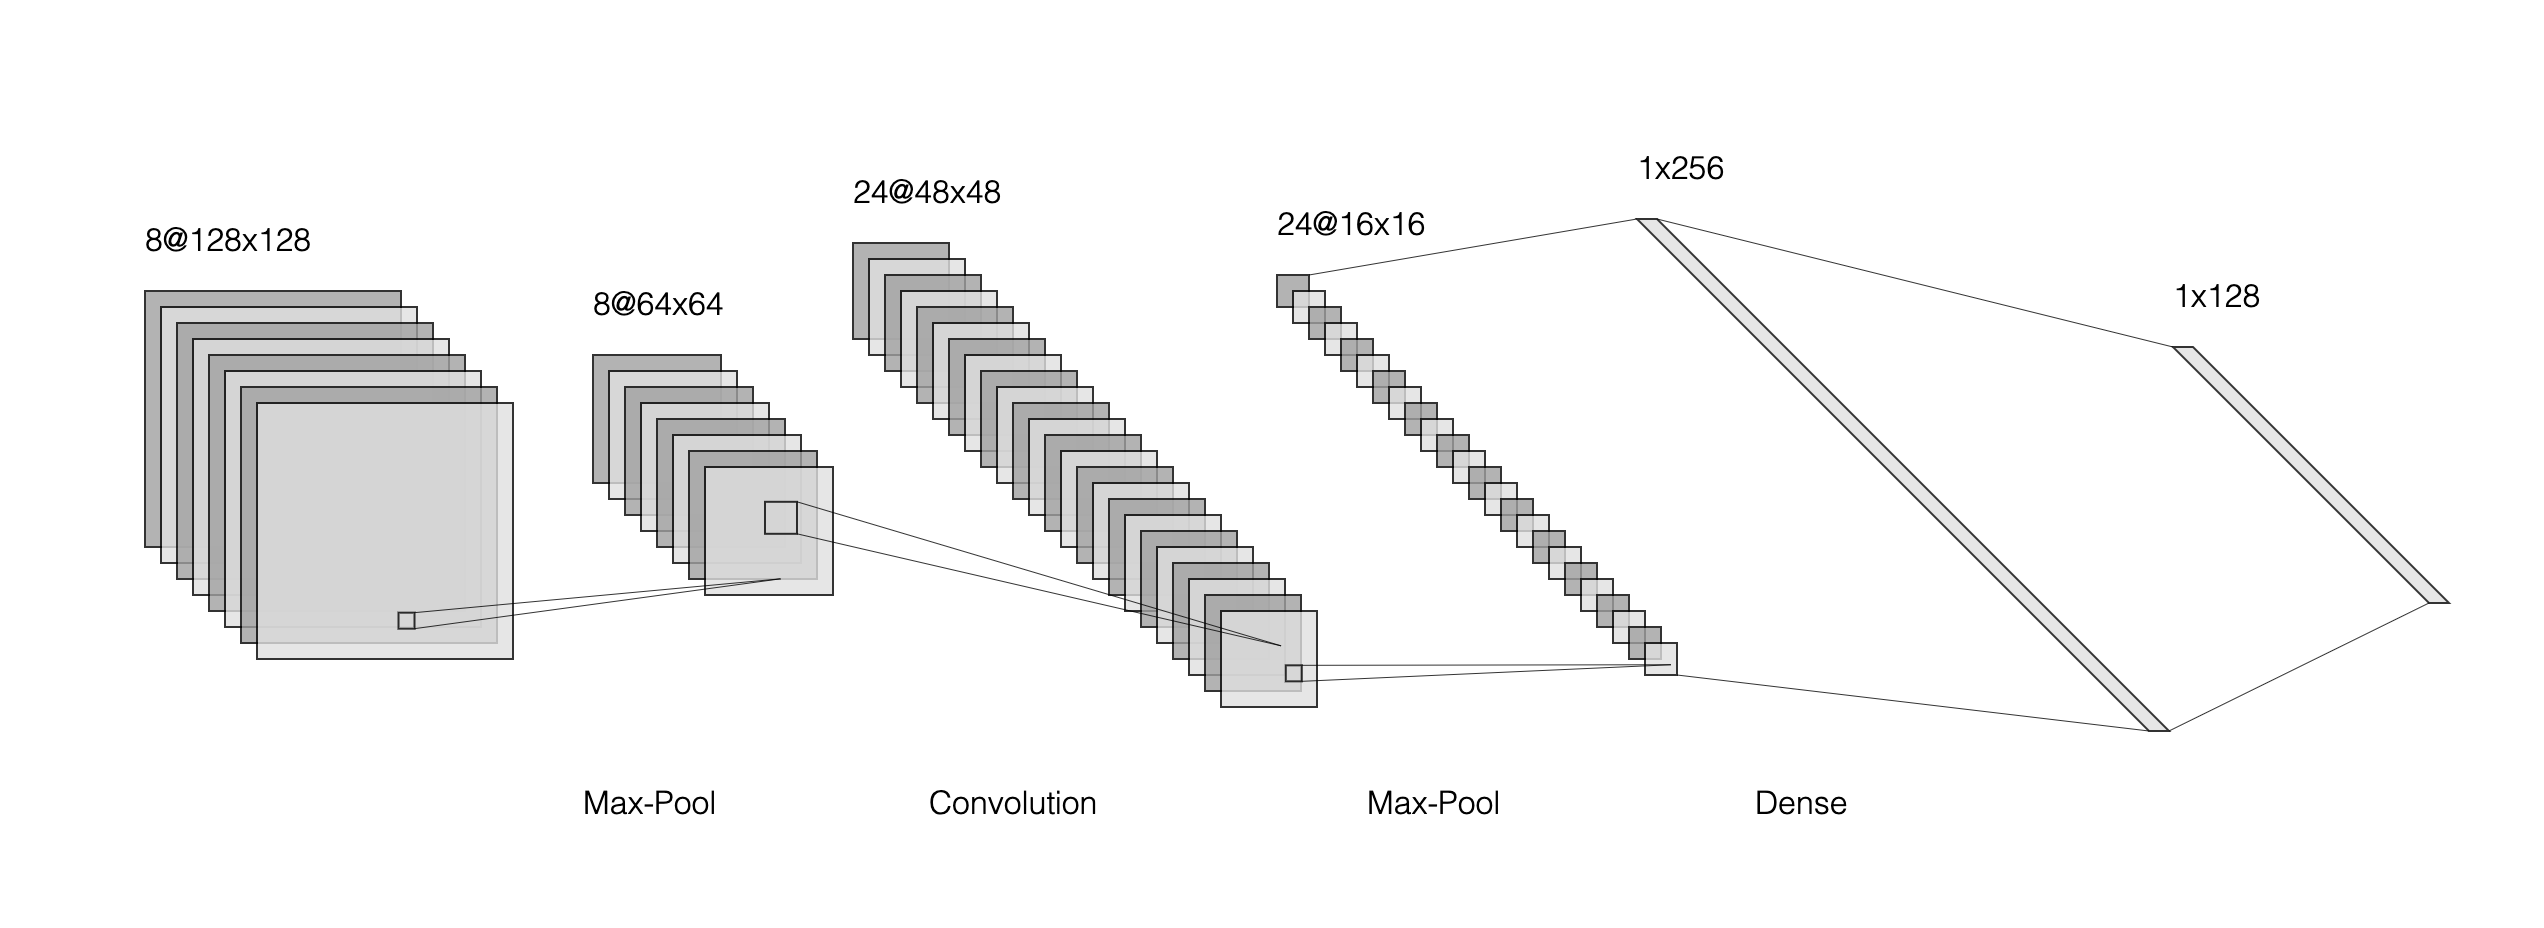
\includegraphics[width=0.75\linewidth,height=\textheight,keepaspectratio]{figures/nn.png}

\subsection{Training Procedure}\label{training-procedure}

\begin{Shaded}
\begin{Highlighting}[]
\ControlFlowTok{for}\NormalTok{ epoch }\KeywordTok{in} \BuiltInTok{range}\NormalTok{(}\DecValTok{10}\NormalTok{):}
\NormalTok{    train\_loss }\OperatorTok{=}\NormalTok{ train\_epoch(model, train\_loader, optimizer)}
    \BuiltInTok{print}\NormalTok{(}\SpecialStringTok{f"Epoch }\SpecialCharTok{\{}\NormalTok{epoch}\SpecialCharTok{\}}\SpecialStringTok{: loss = }\SpecialCharTok{\{}\NormalTok{train\_loss}\SpecialCharTok{:.4f\}}\SpecialStringTok{"}\NormalTok{)}
\end{Highlighting}
\end{Shaded}

\section{Experiments and Results}\label{experiments-and-results}

Insert plot:

\includegraphics[width=0.75\linewidth,height=\textheight,keepaspectratio]{figures/placeholder.png}

Example Table:

\begin{longtable}[]{@{}lll@{}}
\toprule\noalign{}
Experiment & Accuracy (\%) & F1 Score \\
\midrule\noalign{}
\endhead
\bottomrule\noalign{}
\endlastfoot
Baseline & 85 & 0.80 \\
Proposed Model & 90 & 0.88 \\
\end{longtable}

\section{Discussion}\label{discussion}

Summarize key findings and limitations.

\section{Ethical Considerations}\label{ethical-considerations}

Mention privacy, bias, societal impact.

\section{Conclusion and Future Work}\label{conclusion-and-future-work}

\section*{References}\label{references}
\addcontentsline{toc}{section}{References}

\phantomsection\label{refs}

\section*{Appendices}\label{appendices}
\addcontentsline{toc}{section}{Appendices}

\subsection{Libraries Used}\label{libraries-used}

import os import time import random from tqdm import tqdm from selenium
import webdriver from selenium.webdriver.chrome.service import Service
from selenium.webdriver.chrome.options import Options from
selenium.webdriver.common.by import By from
selenium.webdriver.support.ui import WebDriverWait from
selenium.webdriver.support import expected\_conditions as EC from
urllib.parse import quote\_plus

from app.scrape\_logger import ScrapeLogger from app.browser import
Browser, user\_agents

import os import sys import base64 import requests from tqdm import tqdm
import concurrent.futures from bs4 import BeautifulSoup from dotenv
import load\_dotenv from urllib.parse import urlparse

from openai import OpenAI from google import genai from google.genai
import types

from error\_logger import ErrorLogger from extractor import
extract\_text, is\_valid\_website from topics import topic\_dict\_small,
topic\_dict\_medium, topic\_dict\_max

\subsection{Full Code}\label{full-code}

\subsubsection{Webscraper}\label{webscraper}

\begin{Shaded}
\begin{Highlighting}[]
\KeywordTok{def}\NormalTok{ wait\_for\_captcha(browser: Browser, timeout}\OperatorTok{=}\DecValTok{1}\NormalTok{) }\OperatorTok{{-}\textgreater{}} \BuiltInTok{bool}\NormalTok{:}
    \CommentTok{"""}
\CommentTok{    Waits for the ReCAPTCHA element to appear on the page.}
\CommentTok{    Args:}
\CommentTok{        browser (Browser): The Browser instance to use for scraping.}
\CommentTok{        timeout (int): The maximum time to wait for the ReCAPTCHA element to appear.}
\CommentTok{    """}
    \ControlFlowTok{try}\NormalTok{:}
\NormalTok{        WebDriverWait(browser.browser, timeout).until(}
\NormalTok{            EC.presence\_of\_element\_located((By.ID, }\StringTok{"captcha{-}form"}\NormalTok{))}
\NormalTok{        )}
        \BuiltInTok{input}\NormalTok{(}\StringTok{"Please manually complete the authentication, then press Enter to continue..."}\NormalTok{)}
        \ControlFlowTok{return} \VariableTok{True}
    \ControlFlowTok{except}\NormalTok{:}
        \ControlFlowTok{return} \VariableTok{False}
\end{Highlighting}
\end{Shaded}

\begin{Shaded}
\begin{Highlighting}[]
\KeywordTok{def}\NormalTok{ get\_options(chrome\_binary\_path: }\BuiltInTok{str}\NormalTok{, enhanced\_options: }\BuiltInTok{bool} \OperatorTok{=} \VariableTok{False}\NormalTok{) }\OperatorTok{{-}\textgreater{}}\NormalTok{ Options:}
    \CommentTok{"""}
\CommentTok{    Returns Chrome Options class for the browser instance with enhanced }
\CommentTok{    features for resource management and ReCAPTCHA avoidance.}
\CommentTok{    """}
    
    \CommentTok{\# Set up Chrome options}
\NormalTok{    options }\OperatorTok{=}\NormalTok{ Options()}

    \CommentTok{\# Define the binary path for Chrome}
\NormalTok{    options.binary\_location }\OperatorTok{=}\NormalTok{ chrome\_binary\_path}

    \ControlFlowTok{if} \KeywordTok{not}\NormalTok{ enhanced\_options:}
        \ControlFlowTok{return}\NormalTok{ options}
    
    \CommentTok{\# Select a random user agent}
\NormalTok{    random\_user\_agent }\OperatorTok{=}\NormalTok{ random.choice(user\_agents)}

    \CommentTok{\# options.add\_argument("{-}{-}window{-}size=960,640") \# Set a small window size to reduce resource usage}
    \CommentTok{\# options.add\_argument("{-}{-}disable{-}notifications")  \# Prevents notification promp}

    \CommentTok{\# Disable automation flags}
\NormalTok{    options.add\_argument(}\StringTok{"{-}{-}disable{-}blink{-}features=AutomationControlled"}\NormalTok{)}
\NormalTok{    options.add\_experimental\_option(}\StringTok{"excludeSwitches"}\NormalTok{, [}\StringTok{"enable{-}automation"}\NormalTok{])}
\NormalTok{    options.add\_experimental\_option(}\StringTok{"useAutomationExtension"}\NormalTok{, }\VariableTok{False}\NormalTok{)}

    \CommentTok{\# Set the user agent to a random one}
\NormalTok{    options.add\_argument(}\SpecialStringTok{f\textquotesingle{}user{-}agent=}\SpecialCharTok{\{}\NormalTok{random\_user\_agent}\SpecialCharTok{\}}\SpecialStringTok{\textquotesingle{}}\NormalTok{)}

    \ControlFlowTok{return}\NormalTok{ options}
\end{Highlighting}
\end{Shaded}

\begin{Shaded}
\begin{Highlighting}[]
\KeywordTok{def}\NormalTok{ random\_sleep(}\BuiltInTok{long}\NormalTok{: }\BuiltInTok{bool} \OperatorTok{=} \VariableTok{False}\NormalTok{) }\OperatorTok{{-}\textgreater{}} \VariableTok{None}\NormalTok{:}
    \CommentTok{"""}
\CommentTok{    Sleeps for a random duration between 0.5 and 12 seconds or between 10 and 12 seconds.}
\CommentTok{    Args:}
\CommentTok{        long (bool): If True, sleep for a longer duration (10{-}12 seconds). Default is False.}
\CommentTok{    """}
    \ControlFlowTok{if} \BuiltInTok{long}\NormalTok{:}
\NormalTok{        time.sleep(random.uniform(}\DecValTok{10}\NormalTok{, }\DecValTok{18}\NormalTok{))}
    \ControlFlowTok{else}\NormalTok{:}
\NormalTok{        time.sleep(random.uniform(}\FloatTok{0.5}\NormalTok{, }\DecValTok{1}\NormalTok{))}
\end{Highlighting}
\end{Shaded}

\begin{Shaded}
\begin{Highlighting}[]
\KeywordTok{def}\NormalTok{ generate\_search\_urls(filepath: }\BuiltInTok{str}\NormalTok{) }\OperatorTok{{-}\textgreater{}} \BuiltInTok{list}\NormalTok{:}
    \CommentTok{"""}
\CommentTok{    Reads search keywords from a text file and generates Google search URLs.}

\CommentTok{    Args:}
\CommentTok{        filepath (str): The path to the text file containing search keywords.}

\CommentTok{    Returns:}
\CommentTok{        list: A list of Google search URLs.}
\CommentTok{    """}
\NormalTok{    keyword\_to\_url }\OperatorTok{=} \BuiltInTok{dict}\NormalTok{()}
    \ControlFlowTok{try}\NormalTok{:}
        \ControlFlowTok{with} \BuiltInTok{open}\NormalTok{(filepath, }\StringTok{\textquotesingle{}r\textquotesingle{}}\NormalTok{, encoding}\OperatorTok{=}\StringTok{\textquotesingle{}utf{-}8\textquotesingle{}}\NormalTok{) }\ImportTok{as} \BuiltInTok{file}\NormalTok{:}
            \ControlFlowTok{for}\NormalTok{ line }\KeywordTok{in} \BuiltInTok{file}\NormalTok{:}
\NormalTok{                keyword }\OperatorTok{=}\NormalTok{ line.strip()  }\CommentTok{\# Remove newline characters at the end of lines}
                \ControlFlowTok{if}\NormalTok{ keyword:  }\CommentTok{\# Ensure the keyword is not empty}
\NormalTok{                    encoded\_keyword }\OperatorTok{=}\NormalTok{ quote\_plus(keyword)  }\CommentTok{\# URL{-}encode the keyword}
\NormalTok{                    url }\OperatorTok{=} \SpecialStringTok{f\textquotesingle{}https://www.google.com.tw/search?q=}\SpecialCharTok{\{}\NormalTok{encoded\_keyword}\SpecialCharTok{\}}\SpecialStringTok{\textquotesingle{}}
\NormalTok{                    keyword\_to\_url[keyword] }\OperatorTok{=}\NormalTok{ url}
    \ControlFlowTok{except} \PreprocessorTok{FileNotFoundError}\NormalTok{:}
        \BuiltInTok{print}\NormalTok{(}\SpecialStringTok{f"File not found: }\SpecialCharTok{\{}\NormalTok{filepath}\SpecialCharTok{\}}\SpecialStringTok{"}\NormalTok{)}
    \ControlFlowTok{return}\NormalTok{ keyword\_to\_url}
\end{Highlighting}
\end{Shaded}

\begin{Shaded}
\begin{Highlighting}[]
\KeywordTok{def}\NormalTok{ scrape\_url(}
\NormalTok{        browser: Browser, }
\NormalTok{        url: }\BuiltInTok{str}\NormalTok{, }
\NormalTok{        topic: }\BuiltInTok{str}\NormalTok{, }
\NormalTok{        url\_index: }\BuiltInTok{int}\NormalTok{, }
\NormalTok{        max\_pagiation: }\BuiltInTok{int} \OperatorTok{=} \DecValTok{5}\NormalTok{, }
\NormalTok{        pagination\_xpath: }\BuiltInTok{str} \OperatorTok{=} \StringTok{"//td[@class=}\CharTok{\textbackslash{}"}\StringTok{NKTSme}\CharTok{\textbackslash{}"}\StringTok{]/a"}\NormalTok{, }
\NormalTok{        url\_xpath: }\BuiltInTok{str} \OperatorTok{=} \StringTok{"//a[@class=}\CharTok{\textbackslash{}"}\StringTok{zReHs}\CharTok{\textbackslash{}"}\StringTok{]"}\NormalTok{,}
\NormalTok{        logger: ScrapeLogger }\OperatorTok{=} \VariableTok{None}\NormalTok{,}
\NormalTok{        keyword: }\BuiltInTok{str} \OperatorTok{=} \VariableTok{None}
\NormalTok{        ) }\OperatorTok{{-}\textgreater{}} \VariableTok{None}\NormalTok{:}
    \CommentTok{"""}
\CommentTok{    Scrapes URLs from Google search results, handles authentication, and performs pagination.}

\CommentTok{    Args:}
\CommentTok{        browser (Browser): The Browser instance to use for scraping.}
\CommentTok{        url (str): The Google search URL to scrape.}
\CommentTok{        result\_filename (str): The filename to save the scraped results.}
\CommentTok{    """}
    
    \CommentTok{\# Create empty set to store all scraped URLs}
\NormalTok{    all\_scraped\_urls }\OperatorTok{=} \BuiltInTok{set}\NormalTok{()}
\NormalTok{    result\_filename }\OperatorTok{=} \SpecialStringTok{f\textquotesingle{}result/}\SpecialCharTok{\{}\NormalTok{topic}\SpecialCharTok{\}}\SpecialStringTok{.txt\textquotesingle{}}
\NormalTok{    captcha\_count }\OperatorTok{=} \DecValTok{0}
\NormalTok{    captcha\_triggered }\OperatorTok{=} \VariableTok{False}
    
    \CommentTok{\# Open the search URL and wait for captcha}
\NormalTok{    browser.open\_page(url)}

    \CommentTok{\# Wait for captcha}
\NormalTok{    initial\_captcha }\OperatorTok{=}\NormalTok{ wait\_for\_captcha(browser}\OperatorTok{=}\NormalTok{browser)}
    \ControlFlowTok{if}\NormalTok{ initial\_captcha:}
\NormalTok{            captcha\_count }\OperatorTok{+=} \DecValTok{1}
\NormalTok{            captcha\_triggered }\OperatorTok{=} \VariableTok{True}
    
    \CommentTok{\# Long sleep to avoid detection}
\NormalTok{    random\_sleep(}\BuiltInTok{long}\OperatorTok{=}\VariableTok{True}\NormalTok{)}

    \CommentTok{\# Get links for pagiation}
\NormalTok{    pagination\_links }\OperatorTok{=}\NormalTok{ browser.find\_elements(pagination\_xpath)}

    \CommentTok{\# Visit each pagination URL one by one}
    \ControlFlowTok{for}\NormalTok{ i, page\_url }\KeywordTok{in} \BuiltInTok{enumerate}\NormalTok{(pagination\_links):}
    
        \CommentTok{\# Open the pagination URL}
\NormalTok{        browser.open\_page(page\_url)}
        
        \CommentTok{\# Check for captcha}
\NormalTok{        captcha\_flag }\OperatorTok{=}\NormalTok{ wait\_for\_captcha(browser}\OperatorTok{=}\NormalTok{browser)}

        \CommentTok{\# update captcha count and triggered status}
        \ControlFlowTok{if}\NormalTok{ captcha\_flag:}
\NormalTok{            captcha\_count }\OperatorTok{+=} \DecValTok{1}
\NormalTok{            captcha\_triggered }\OperatorTok{=}\NormalTok{ captcha\_triggered }\KeywordTok{or}\NormalTok{ captcha\_flag}

        \CommentTok{\# browser.random\_scroll()}
        \CommentTok{\# Extract URLs from the current page}
\NormalTok{        random\_sleep(}\BuiltInTok{long}\OperatorTok{=}\VariableTok{False}\NormalTok{)}
\NormalTok{        extracted\_urls }\OperatorTok{=}\NormalTok{ browser.find\_elements(url\_xpath)}
\NormalTok{        all\_scraped\_urls.update(extracted\_urls)}

        \ControlFlowTok{if}\NormalTok{ i }\OperatorTok{\textgreater{}=}\NormalTok{ max\_pagiation:}
            \ControlFlowTok{break}

\NormalTok{    browser.save\_urls\_to\_file(all\_scraped\_urls, result\_filename)}
\NormalTok{    logger.log\_url\_scrape(}
\NormalTok{        keyword}\OperatorTok{=}\NormalTok{keyword, }
\NormalTok{        url\_idx}\OperatorTok{=}\NormalTok{url\_index, }
\NormalTok{        captcha\_present}\OperatorTok{=}\NormalTok{captcha\_triggered,  }\CommentTok{\# Assuming captcha was handled manually}
\NormalTok{        captcha\_count}\OperatorTok{=}\NormalTok{captcha\_count,  }\CommentTok{\# Assuming no captcha count for this URL}
\NormalTok{        num\_extracted}\OperatorTok{=}\BuiltInTok{len}\NormalTok{(all\_scraped\_urls)}
\NormalTok{    )}
\end{Highlighting}
\end{Shaded}

\begin{Shaded}
\begin{Highlighting}[]
\KeywordTok{def}\NormalTok{ main():}
    \CommentTok{\# Define the paths to ChromeDriver and Chrome binary}
\NormalTok{    driver\_path }\OperatorTok{=} \StringTok{\textquotesingle{}/opt/homebrew/bin/chromedriver\textquotesingle{}}  \CommentTok{\# Replace with your ChromeDriver path}
\NormalTok{    chrome\_binary\_path }\OperatorTok{=} \StringTok{"/Applications/Google Chrome.app/Contents/MacOS/Google Chrome"}  \CommentTok{\# For defining browser options}

\NormalTok{    pagiation\_xpath }\OperatorTok{=} \StringTok{"//td[@class=}\CharTok{\textbackslash{}"}\StringTok{NKTSme}\CharTok{\textbackslash{}"}\StringTok{]/a"}
\NormalTok{    url\_xpath }\OperatorTok{=} \StringTok{"//a[@class=}\CharTok{\textbackslash{}"}\StringTok{zReHs}\CharTok{\textbackslash{}"}\StringTok{]"}
\NormalTok{    max\_pagiation }\OperatorTok{=} \DecValTok{5}
\NormalTok{    broser\_reset\_interval }\OperatorTok{=} \DecValTok{5}

    \CommentTok{\# Ask for the keyword file to scrape}
\NormalTok{    topic }\OperatorTok{=} \BuiltInTok{str}\NormalTok{(}\BuiltInTok{input}\NormalTok{(}\StringTok{"Enter the category you would like to scrape: "}\NormalTok{))}
\NormalTok{    start\_url\_idx }\OperatorTok{=} \BuiltInTok{input}\NormalTok{(}\StringTok{"Enter the starting URL index (0 for first): "}\NormalTok{)}
\NormalTok{    start\_index }\OperatorTok{=} \BuiltInTok{int}\NormalTok{(start\_url\_idx) }\ControlFlowTok{if}\NormalTok{ start\_url\_idx.strip() }\ControlFlowTok{else} \DecValTok{0}

    \CommentTok{\# Check if the keyword file exists and define the search URL keywords}
\NormalTok{    keyword\_filepath }\OperatorTok{=} \SpecialStringTok{f\textquotesingle{}keyword/}\SpecialCharTok{\{}\NormalTok{topic}\SpecialCharTok{\}}\SpecialStringTok{.txt\textquotesingle{}}
    \ControlFlowTok{if} \KeywordTok{not}\NormalTok{ os.path.exists(keyword\_filepath):}
        \BuiltInTok{print}\NormalTok{(}\SpecialStringTok{f"File not found: }\SpecialCharTok{\{}\NormalTok{keyword\_filepath}\SpecialCharTok{\}}\SpecialStringTok{"}\NormalTok{)}
        \ControlFlowTok{return}

    \CommentTok{\# Generate search URLs from the keyword file}
\NormalTok{    search\_url\_dict }\OperatorTok{=}\NormalTok{ generate\_search\_urls(keyword\_filepath)}
    
    \CommentTok{\# define browser options, create browser instance, define the logger}
\NormalTok{    options }\OperatorTok{=}\NormalTok{ get\_options(chrome\_binary\_path}\OperatorTok{=}\NormalTok{chrome\_binary\_path)}
\NormalTok{    browser }\OperatorTok{=}\NormalTok{ Browser(driver\_path, options)}

    \CommentTok{\# Create the logger instance}
\NormalTok{    logger }\OperatorTok{=}\NormalTok{ ScrapeLogger(topic}\OperatorTok{=}\NormalTok{topic)}

    \ControlFlowTok{for}\NormalTok{ i, keyword }\KeywordTok{in}\NormalTok{ tqdm(}
        \BuiltInTok{enumerate}\NormalTok{(search\_url\_dict),}
\NormalTok{        total}\OperatorTok{=}\BuiltInTok{len}\NormalTok{(search\_url\_dict),}
\NormalTok{        desc}\OperatorTok{=}\StringTok{"Scraping URLs"}\NormalTok{,}
\NormalTok{        unit}\OperatorTok{=}\StringTok{"url"}\NormalTok{,}
\NormalTok{        leave}\OperatorTok{=}\VariableTok{True}
\NormalTok{    ):}
        \ControlFlowTok{if}\NormalTok{ i }\OperatorTok{\textless{}}\NormalTok{ start\_index:}
            \ControlFlowTok{continue}

\NormalTok{        url }\OperatorTok{=}\NormalTok{ search\_url\_dict[keyword]}
        \CommentTok{\# Scrape URLs from the search results }
\NormalTok{        scrape\_url(}
\NormalTok{            browser}\OperatorTok{=}\NormalTok{browser, }
\NormalTok{            url}\OperatorTok{=}\NormalTok{url, }
\NormalTok{            topic}\OperatorTok{=}\NormalTok{topic, }
\NormalTok{            url\_index}\OperatorTok{=}\NormalTok{i, }
\NormalTok{            max\_pagiation}\OperatorTok{=}\NormalTok{max\_pagiation, }
\NormalTok{            pagination\_xpath}\OperatorTok{=}\NormalTok{pagiation\_xpath, }
\NormalTok{            url\_xpath}\OperatorTok{=}\NormalTok{url\_xpath, }
\NormalTok{            logger}\OperatorTok{=}\NormalTok{logger,}
\NormalTok{            keyword}\OperatorTok{=}\NormalTok{keyword}
\NormalTok{        )}

        \CommentTok{\# Random sleep to avoid detection}
\NormalTok{        random\_sleep(}\BuiltInTok{long}\OperatorTok{=}\VariableTok{True}\NormalTok{)}

        \ControlFlowTok{if}\NormalTok{ i }\OperatorTok{\%}\NormalTok{ broser\_reset\_interval }\OperatorTok{==}\NormalTok{ (broser\_reset\_interval }\OperatorTok{{-}} \DecValTok{1}\NormalTok{):}
            \CommentTok{\# Close the browser to avoid detection}
\NormalTok{            browser.close\_browser()}
\NormalTok{            random\_sleep(}\BuiltInTok{long}\OperatorTok{=}\VariableTok{True}\NormalTok{)}

            \CommentTok{\# Recreate the browser instance}
\NormalTok{            browser }\OperatorTok{=}\NormalTok{ Browser(driver\_path, options)}

\NormalTok{    browser.close\_browser()}
\NormalTok{    logger.log\_end()}

\ControlFlowTok{if} \VariableTok{\_\_name\_\_} \OperatorTok{==} \StringTok{"\_\_main\_\_"}\NormalTok{:}
\NormalTok{    main()}
\end{Highlighting}
\end{Shaded}

\subsubsection{Website Labeler}\label{website-labeler}

\begin{Shaded}
\begin{Highlighting}[]
\CommentTok{\# Create a global Gemini client to reuse}
\NormalTok{client }\OperatorTok{=} \VariableTok{None}

\KeywordTok{def}\NormalTok{ initialize\_client():}
    \KeywordTok{global}\NormalTok{ client}
    \ControlFlowTok{if}\NormalTok{ client }\KeywordTok{is} \VariableTok{None}\NormalTok{:}
\NormalTok{        client }\OperatorTok{=}\NormalTok{ genai.Client(api\_key}\OperatorTok{=}\NormalTok{os.environ.get(}\StringTok{"GOOGLE\_API\_KEY"}\NormalTok{))}
    \ControlFlowTok{return}\NormalTok{ client}
\end{Highlighting}
\end{Shaded}

\begin{Shaded}
\begin{Highlighting}[]
\KeywordTok{def}\NormalTok{ is\_valid\_website(url: }\BuiltInTok{str} \OperatorTok{=} \StringTok{""}\NormalTok{, error\_logger: ErrorLogger }\OperatorTok{=} \VariableTok{None}\NormalTok{):}
    \CommentTok{"""Check if the website responds successfully."""}
    \CommentTok{\# Add scheme if missing}
    \ControlFlowTok{if} \KeywordTok{not}\NormalTok{ url.startswith((}\StringTok{\textquotesingle{}http://\textquotesingle{}}\NormalTok{, }\StringTok{\textquotesingle{}https://\textquotesingle{}}\NormalTok{)):}
\NormalTok{        url }\OperatorTok{=} \StringTok{\textquotesingle{}https://\textquotesingle{}} \OperatorTok{+}\NormalTok{ url}
    
\NormalTok{    headers }\OperatorTok{=}\NormalTok{ \{}
        \StringTok{\textquotesingle{}User{-}Agent\textquotesingle{}}\NormalTok{: }\StringTok{\textquotesingle{}Mozilla/5.0 (Windows NT 10.0; Win64; x64) AppleWebKit/537.36 (KHTML, like Gecko) Chrome/91.0.4472.124 Safari/537.36\textquotesingle{}}
\NormalTok{    \}}
    
    \ControlFlowTok{try}\NormalTok{:}
\NormalTok{        response }\OperatorTok{=}\NormalTok{ requests.get(}
\NormalTok{            url,}
\NormalTok{            headers}\OperatorTok{=}\NormalTok{headers,}
\NormalTok{            timeout}\OperatorTok{=}\DecValTok{10}\NormalTok{,}
\NormalTok{            allow\_redirects}\OperatorTok{=}\VariableTok{True}
\NormalTok{        )}
        
        \CommentTok{\# Consider 2xx and 3xx status codes as valid}
        \ControlFlowTok{return} \DecValTok{200} \OperatorTok{\textless{}=}\NormalTok{ response.status\_code }\OperatorTok{\textless{}} \DecValTok{400}\NormalTok{, response.status\_code}
        
    \ControlFlowTok{except}\NormalTok{ requests.RequestException }\ImportTok{as}\NormalTok{ e:}
        \CommentTok{\# Try HTTP if HTTPS failed}
        \ControlFlowTok{if}\NormalTok{ url.startswith(}\StringTok{\textquotesingle{}https://\textquotesingle{}}\NormalTok{):}
            \ControlFlowTok{try}\NormalTok{:}
\NormalTok{                http\_url }\OperatorTok{=} \StringTok{\textquotesingle{}http://\textquotesingle{}} \OperatorTok{+}\NormalTok{ url[}\DecValTok{8}\NormalTok{:]}
\NormalTok{                response }\OperatorTok{=}\NormalTok{ requests.get(}
\NormalTok{                    http\_url,}
\NormalTok{                    headers}\OperatorTok{=}\NormalTok{headers,}
\NormalTok{                    timeout}\OperatorTok{=}\DecValTok{10}\NormalTok{,}
\NormalTok{                    allow\_redirects}\OperatorTok{=}\VariableTok{True}
\NormalTok{                )}
                \ControlFlowTok{if} \DecValTok{200} \OperatorTok{\textless{}=}\NormalTok{ response.status\_code }\OperatorTok{\textless{}} \DecValTok{400}\NormalTok{:}
                    \ControlFlowTok{return} \VariableTok{True}\NormalTok{, response.status\_code}
            \ControlFlowTok{except}\NormalTok{:}
                \ControlFlowTok{pass}
                
        \ControlFlowTok{if}\NormalTok{ error\_logger:}
\NormalTok{            error\_logger.log\_error(}\StringTok{"connection"}\NormalTok{, url, }\SpecialStringTok{f"Connection error: }\SpecialCharTok{\{}\NormalTok{e}\SpecialCharTok{\}}\SpecialStringTok{"}\NormalTok{)}
        \ControlFlowTok{return} \VariableTok{False}
\end{Highlighting}
\end{Shaded}

\begin{Shaded}
\begin{Highlighting}[]
\KeywordTok{def}\NormalTok{ extract\_text(url: }\BuiltInTok{str} \OperatorTok{=} \StringTok{""}\NormalTok{, error\_logger: ErrorLogger }\OperatorTok{=} \VariableTok{None}\NormalTok{):}
    \CommentTok{"""Extracts text content from a website."""}
    \ControlFlowTok{try}\NormalTok{:}
\NormalTok{        response }\OperatorTok{=}\NormalTok{ requests.get(url, timeout}\OperatorTok{=}\DecValTok{10}\NormalTok{)}
        \ControlFlowTok{if} \KeywordTok{not}\NormalTok{ response.encoding:}
\NormalTok{            response.encoding }\OperatorTok{=} \StringTok{\textquotesingle{}utf{-}8\textquotesingle{}}
\NormalTok{        soup }\OperatorTok{=}\NormalTok{ BeautifulSoup(response.text, }\StringTok{\textquotesingle{}html.parser\textquotesingle{}}\NormalTok{)}

        \CommentTok{\# Extract text from common tags}
\NormalTok{        texts }\OperatorTok{=}\NormalTok{ []}
        \ControlFlowTok{for}\NormalTok{ tag }\KeywordTok{in}\NormalTok{ soup.find\_all([}\StringTok{\textquotesingle{}p\textquotesingle{}}\NormalTok{, }\StringTok{\textquotesingle{}span\textquotesingle{}}\NormalTok{, }\StringTok{\textquotesingle{}h1\textquotesingle{}}\NormalTok{, }\StringTok{\textquotesingle{}h2\textquotesingle{}}\NormalTok{, }\StringTok{\textquotesingle{}h3\textquotesingle{}}\NormalTok{, }\StringTok{\textquotesingle{}h4\textquotesingle{}}\NormalTok{]):}
\NormalTok{            texts.append(tag.get\_text(separator}\OperatorTok{=}\StringTok{\textquotesingle{} \textquotesingle{}}\NormalTok{, strip}\OperatorTok{=}\VariableTok{True}\NormalTok{))}
\NormalTok{        combined\_text }\OperatorTok{=} \StringTok{\textquotesingle{} \textquotesingle{}}\NormalTok{.join(texts)}
        \ControlFlowTok{if}\NormalTok{ combined\_text:}
            \ControlFlowTok{return}\NormalTok{ combined\_text[:}\DecValTok{40000}\NormalTok{]}

        \CommentTok{\# Fallback: extract from the entire body}
        \ControlFlowTok{if}\NormalTok{ soup.body:}
\NormalTok{            text }\OperatorTok{=}\NormalTok{ soup.body.get\_text(separator}\OperatorTok{=}\StringTok{\textquotesingle{} \textquotesingle{}}\NormalTok{, strip}\OperatorTok{=}\VariableTok{True}\NormalTok{)}
            \ControlFlowTok{return}\NormalTok{ text[:}\DecValTok{40000}\NormalTok{]}

    \ControlFlowTok{except}\NormalTok{ requests.RequestException }\ImportTok{as}\NormalTok{ e:}
        \ControlFlowTok{if}\NormalTok{ error\_logger:}
\NormalTok{            error\_logger.log\_error(}\StringTok{"parsing"}\NormalTok{, url, }\SpecialStringTok{f"Content extraction error: }\SpecialCharTok{\{}\NormalTok{e}\SpecialCharTok{\}}\SpecialStringTok{"}\NormalTok{)}
        \ControlFlowTok{return} \VariableTok{None}
    \ControlFlowTok{except} \PreprocessorTok{Exception} \ImportTok{as}\NormalTok{ e:}
        \ControlFlowTok{if}\NormalTok{ error\_logger:}
\NormalTok{            error\_logger.log\_error(}\StringTok{"parsing"}\NormalTok{, url, }\SpecialStringTok{f"HTML parsing error: }\SpecialCharTok{\{}\NormalTok{e}\SpecialCharTok{\}}\SpecialStringTok{"}\NormalTok{)}
        \ControlFlowTok{return} \VariableTok{None}
    \ControlFlowTok{return} \VariableTok{None}
\end{Highlighting}
\end{Shaded}

\begin{Shaded}
\begin{Highlighting}[]
\KeywordTok{def}\NormalTok{ classify\_website(}
\NormalTok{    content: }\BuiltInTok{str}\NormalTok{, }
\NormalTok{    topic: }\BuiltInTok{str}\NormalTok{, }
\NormalTok{    url\_type: }\BuiltInTok{str} \OperatorTok{=} \StringTok{"{-}"}\NormalTok{, }
\NormalTok{    url: }\BuiltInTok{str} \OperatorTok{=} \StringTok{""}\NormalTok{, }
\NormalTok{    error\_logger: ErrorLogger }\OperatorTok{=} \VariableTok{None}\NormalTok{, }
\NormalTok{    host\_flag: }\BuiltInTok{bool} \OperatorTok{=} \VariableTok{False}\NormalTok{):}
    \CommentTok{"""Uses the Gemini model to classify website content."""}

\NormalTok{    topics\_dict }\OperatorTok{=}\NormalTok{ topic\_dict\_medium}

    \ControlFlowTok{if}\NormalTok{ topic }\KeywordTok{not} \KeywordTok{in}\NormalTok{ topics\_dict:}
        \ControlFlowTok{if}\NormalTok{ error\_logger }\KeywordTok{and}\NormalTok{ url:}
\NormalTok{            error\_logger.log\_error(}\StringTok{"configuration"}\NormalTok{, url, }\SpecialStringTok{f"Unknown topic: }\SpecialCharTok{\{}\NormalTok{topic}\SpecialCharTok{\}}\SpecialStringTok{"}\NormalTok{)}
        \CommentTok{\# print("checkpoint 1")}
        \ControlFlowTok{return} \StringTok{\textquotesingle{}u\textquotesingle{}}  \CommentTok{\# Default to \textquotesingle{}unrelated\textquotesingle{}}

\NormalTok{    prompt }\OperatorTok{=} \SpecialStringTok{f"""}
\SpecialStringTok{    You are a specialized content classifier analyzing Chinese website content for sensitive/restricted topics with cultural awareness.}
\SpecialStringTok{    We are designing a website classifier for Chinese websites that is designed to filter out harmful content for children.}

\SpecialStringTok{    CLASSIFICATION TASK:}
\SpecialStringTok{    Determine if the website content relates to: }\SpecialCharTok{\{}\NormalTok{topics\_dict}\SpecialCharTok{.}\NormalTok{get(topic)}\SpecialCharTok{\}}

\SpecialStringTok{    INSTRUCTIONS:}
\SpecialStringTok{    {-} Analyze entire content structure including titles, headings, links, body text, and metadata}
\SpecialStringTok{    {-} Identify both explicit mentions and implicit references using:}
\SpecialStringTok{        {-} Contextual semantic relationships between phrases}
\SpecialStringTok{        {-} Cultural{-}specific phrasing patterns in Simplified/Traditional Chinese}
\SpecialStringTok{    {-} Consider the website\textquotesingle{}s overall theme and purpose}
\SpecialStringTok{    {-} Flag content that attempts to disguise topics through:}
\SpecialStringTok{        {-} Mixed neutral/harmful phrasing}
\SpecialStringTok{        {-} Obfuscated terminology}
\SpecialStringTok{        {-} Cultural context switching}
\SpecialStringTok{    }
\SpecialStringTok{    CAUTIONS:}
\SpecialStringTok{    {-} Avoid keyword over{-}reliance {-} analyze full contextual meaning}
\SpecialStringTok{    {-} Mark ambiguous cases as "u" (unrellated) if not clear}

\SpecialStringTok{    {-} Also mark the following as "u":}
\SpecialStringTok{        {-} Non{-}Chinese content (Japanese, Korean, English etc.)}
\SpecialStringTok{            {-} Note that Japanese will have Kanji that are Chinese }
\SpecialStringTok{            characters, but the website is in fact Japanese}
\SpecialStringTok{        {-} Pages that focus on non{-}text content (websites such as youtube, tiktok, etc.)}

\SpecialStringTok{    RESPONSE FORMAT AND CRITERIA:}
\SpecialStringTok{    {-} "}\SpecialCharTok{\{}\NormalTok{url\_type}\SpecialCharTok{\}}\SpecialStringTok{" ONLY if ≥70\% confidence based on contextual evidence}
\SpecialStringTok{    {-} "u" for neutral content, unrelated cases, or insufficient evidence}

\SpecialStringTok{    WEBSITE CONTENT:}
\SpecialStringTok{    }\SpecialCharTok{\{}\NormalTok{content}\SpecialCharTok{\}}
\SpecialStringTok{    """}

\NormalTok{    host\_additional\_instructions }\OperatorTok{=} \StringTok{"""}
\StringTok{    ADDITIONAL INSTRUCTIONS FOR HOSTS:}
\StringTok{    Mark the folllowing websites as "u" (unrelated)}
\StringTok{    {-} General information websites such as }
\StringTok{        {-} News outlet homepages}
\StringTok{        {-} Genearic Health websites}
\StringTok{        {-} Lawyer pages }
\StringTok{    """}

    \ControlFlowTok{if}\NormalTok{ host\_flag:}
\NormalTok{        prompt }\OperatorTok{+=}\NormalTok{ host\_additional\_instructions}

    \CommentTok{\# Initialize the client}
\NormalTok{    client }\OperatorTok{=}\NormalTok{ initialize\_client()}

    \CommentTok{\# Define the model }
\NormalTok{    model }\OperatorTok{=} \StringTok{"gemini{-}2.0{-}flash"}

    \CommentTok{\# Generate content to feed to the model}
\NormalTok{    contents }\OperatorTok{=}\NormalTok{ [}
\NormalTok{        types.Content(}
\NormalTok{            role}\OperatorTok{=}\StringTok{"user"}\NormalTok{,}
\NormalTok{            parts}\OperatorTok{=}\NormalTok{[}
\NormalTok{                types.Part.from\_text(text}\OperatorTok{=}\NormalTok{prompt),}
\NormalTok{            ],}
\NormalTok{        ),}
\NormalTok{    ]}

    \CommentTok{\# Define the configuration for the model}
\NormalTok{    generate\_content\_config }\OperatorTok{=}\NormalTok{ types.GenerateContentConfig(}
\NormalTok{        temperature}\OperatorTok{=}\FloatTok{0.1}\NormalTok{,}
\NormalTok{        max\_output\_tokens}\OperatorTok{=}\DecValTok{1}\NormalTok{,}
\NormalTok{        response\_mime\_type}\OperatorTok{=}\StringTok{"text/plain"}\NormalTok{,}
\NormalTok{    )}

    \CommentTok{\# Feed into the model and request a response}
    \ControlFlowTok{try}\NormalTok{:}
        \ControlFlowTok{for}\NormalTok{ chunk }\KeywordTok{in}\NormalTok{ client.models.generate\_content\_stream(}
\NormalTok{            model}\OperatorTok{=}\NormalTok{model,}
\NormalTok{            contents}\OperatorTok{=}\NormalTok{contents,}
\NormalTok{            config}\OperatorTok{=}\NormalTok{generate\_content\_config,}
\NormalTok{        ):}
            \CommentTok{\# Decode the response}
\NormalTok{            result }\OperatorTok{=}\NormalTok{ chunk.text.strip().lower()}

            \CommentTok{\# Check if the result is one of the expected labels}
            \CommentTok{\# h for host, p for page, u for unrelated}
            \ControlFlowTok{if}\NormalTok{ result }\KeywordTok{in}\NormalTok{ [}\StringTok{\textquotesingle{}h\textquotesingle{}}\NormalTok{, }\StringTok{\textquotesingle{}u\textquotesingle{}}\NormalTok{, }\StringTok{\textquotesingle{}p\textquotesingle{}}\NormalTok{]:}
                \CommentTok{\# print(f"checkpoint 2, result: \{result\}")}
                \ControlFlowTok{return}\NormalTok{ result}

    \ControlFlowTok{except} \PreprocessorTok{Exception} \ImportTok{as}\NormalTok{ e:}
        \ControlFlowTok{if}\NormalTok{ error\_logger }\KeywordTok{and}\NormalTok{ url:}
\NormalTok{            error\_logger.log\_error(}\StringTok{"api"}\NormalTok{, url, }\SpecialStringTok{f"Gemini API error: }\SpecialCharTok{\{}\NormalTok{e}\SpecialCharTok{\}}\SpecialStringTok{"}\NormalTok{)}
        \CommentTok{\# print(f"checkpoint 3, error: \{e\}")}
        \ControlFlowTok{return} \StringTok{\textquotesingle{}a\textquotesingle{}}  \CommentTok{\# Default to \textquotesingle{}a\textquotesingle{} in case of an AI related error}
\end{Highlighting}
\end{Shaded}

\begin{Shaded}
\begin{Highlighting}[]
\KeywordTok{def}\NormalTok{ process\_url(}
\NormalTok{    url: }\BuiltInTok{str} \OperatorTok{=} \StringTok{""}\NormalTok{, }
\NormalTok{    topic: }\BuiltInTok{str} \OperatorTok{=} \StringTok{""}\NormalTok{, }
\NormalTok{    url\_type: }\BuiltInTok{str} \OperatorTok{=} \StringTok{"{-}"}\NormalTok{, }
\NormalTok{    error\_logger: ErrorLogger }\OperatorTok{=} \VariableTok{None}\NormalTok{,}
\NormalTok{    host\_flag: }\BuiltInTok{bool} \OperatorTok{=} \VariableTok{False}
\NormalTok{        ):}
    \CommentTok{"""Process a single URL and return the result."""}
    \CommentTok{\# Ensure the URL has a valid scheme}
\NormalTok{    parsed\_url }\OperatorTok{=}\NormalTok{ urlparse(url)}
    \ControlFlowTok{if} \KeywordTok{not}\NormalTok{ parsed\_url.scheme:}
\NormalTok{        url }\OperatorTok{=} \SpecialStringTok{f"http://}\SpecialCharTok{\{}\NormalTok{url}\SpecialCharTok{\}}\SpecialStringTok{"}
    
    \ControlFlowTok{try}\NormalTok{:}
        \ControlFlowTok{if} \KeywordTok{not}\NormalTok{ is\_valid\_website(}
\NormalTok{            url}\OperatorTok{=}\NormalTok{url, }
\NormalTok{            error\_logger}\OperatorTok{=}\NormalTok{error\_logger}
\NormalTok{            ):}
            \CommentTok{\# print("checkpoint 5, invalid website")}
            \ControlFlowTok{return}\NormalTok{ url, }\StringTok{\textquotesingle{}i\textquotesingle{}} \CommentTok{\# Invalid website, return \textquotesingle{}i\textquotesingle{}}

        \ControlFlowTok{else}\NormalTok{: }\CommentTok{\# try to extract content}
\NormalTok{            content }\OperatorTok{=}\NormalTok{ extract\_text(}
\NormalTok{                url}\OperatorTok{=}\NormalTok{url,}
\NormalTok{                error\_logger}\OperatorTok{=}\NormalTok{error\_logger}
\NormalTok{            )}
            \ControlFlowTok{if}\NormalTok{ content: }\CommentTok{\# if content is extracted}
\NormalTok{                label }\OperatorTok{=}\NormalTok{ classify\_website(}
\NormalTok{                    content}\OperatorTok{=}\NormalTok{content,}
\NormalTok{                    topic}\OperatorTok{=}\NormalTok{topic,}
\NormalTok{                    url\_type}\OperatorTok{=}\NormalTok{url\_type,}
\NormalTok{                    url}\OperatorTok{=}\NormalTok{url,}
\NormalTok{                    error\_logger}\OperatorTok{=}\NormalTok{error\_logger,}
\NormalTok{                    host\_flag}\OperatorTok{=}\NormalTok{host\_flag}
\NormalTok{                )}
            \ControlFlowTok{else}\NormalTok{: }\CommentTok{\# If no content is extracted}
                \CommentTok{\# print("checkpoint 6, no content")}
\NormalTok{                label }\OperatorTok{=} \StringTok{\textquotesingle{}b\textquotesingle{}}
        \ControlFlowTok{return}\NormalTok{ url, label}

    \ControlFlowTok{except} \PreprocessorTok{Exception} \ImportTok{as}\NormalTok{ e:}
\NormalTok{        error\_logger.log\_error(}\StringTok{"processing"}\NormalTok{, url, }\SpecialStringTok{f"Unexpected error: }\SpecialCharTok{\{}\NormalTok{e}\SpecialCharTok{\}}\SpecialStringTok{"}\NormalTok{)}
        \CommentTok{\# print("checkpoint 7, error: ", e)}
        \ControlFlowTok{return}\NormalTok{ url, }\StringTok{\textquotesingle{}i\textquotesingle{}}
\end{Highlighting}
\end{Shaded}

\begin{Shaded}
\begin{Highlighting}[]
\KeywordTok{def}\NormalTok{ process\_file(}
\NormalTok{    input\_filename: }\BuiltInTok{str} \OperatorTok{=} \StringTok{""}\NormalTok{, }
\NormalTok{    output\_directory: }\BuiltInTok{str} \OperatorTok{=} \StringTok{"results"}\NormalTok{,}
\NormalTok{    url\_type: }\BuiltInTok{str} \OperatorTok{=} \StringTok{"{-}"}\NormalTok{, }
\NormalTok{    error\_logger: ErrorLogger }\OperatorTok{=} \VariableTok{None}\NormalTok{, }
\NormalTok{    host\_flag: }\BuiltInTok{bool} \OperatorTok{=} \VariableTok{False}\NormalTok{, }
\NormalTok{    max\_workers: }\BuiltInTok{int} \OperatorTok{=} \DecValTok{50}
\NormalTok{        ):}
    \CommentTok{"""}
\CommentTok{    Processes an input TXT file where each line is a URL.}
\CommentTok{    Uses ThreadPoolExecutor for parallel processing.}
\CommentTok{    """}

    \ControlFlowTok{if} \KeywordTok{not}\NormalTok{ host\_flag:}
\NormalTok{        input\_file }\OperatorTok{=}\NormalTok{ os.path.join(}\StringTok{"raw/urls"}\NormalTok{, input\_filename)}
    \ControlFlowTok{else}\NormalTok{:}
\NormalTok{        input\_file }\OperatorTok{=}\NormalTok{ os.path.join(}\StringTok{"raw/hosts"}\NormalTok{, input\_filename)}
    
    \CommentTok{\# Read URLs from file}
    \ControlFlowTok{with} \BuiltInTok{open}\NormalTok{(input\_file, }\StringTok{\textquotesingle{}r\textquotesingle{}}\NormalTok{, encoding}\OperatorTok{=}\StringTok{\textquotesingle{}utf{-}8\textquotesingle{}}\NormalTok{) }\ImportTok{as}\NormalTok{ f:}
\NormalTok{        urls }\OperatorTok{=}\NormalTok{ [line.strip() }\ControlFlowTok{for}\NormalTok{ line }\KeywordTok{in}\NormalTok{ f }\ControlFlowTok{if}\NormalTok{ line.strip()]}
    
    \CommentTok{\# Initialize results list}
\NormalTok{    results }\OperatorTok{=}\NormalTok{ []}
    
    \CommentTok{\# Use a ThreadPoolExecutor for parallel processing}
    \ControlFlowTok{with}\NormalTok{ concurrent.futures.ThreadPoolExecutor(max\_workers}\OperatorTok{=}\NormalTok{max\_workers) }\ImportTok{as}\NormalTok{ executor:}
        \CommentTok{\# Submit all tasks and create a mapping of futures to URLs}
\NormalTok{        future\_to\_url }\OperatorTok{=}\NormalTok{ \{executor.submit(process\_url, url, topic, url\_type, error\_logger, host\_flag): url }\ControlFlowTok{for}\NormalTok{ url }\KeywordTok{in}\NormalTok{ urls\}}
        
        \CommentTok{\# Process results as they complete}
        \ControlFlowTok{for}\NormalTok{ future }\KeywordTok{in}\NormalTok{ tqdm(}
\NormalTok{            concurrent.futures.as\_completed(future\_to\_url),}
\NormalTok{            total}\OperatorTok{=}\BuiltInTok{len}\NormalTok{(urls),}
\NormalTok{            desc}\OperatorTok{=}\StringTok{"Processing URLs"}\NormalTok{,}
\NormalTok{            unit}\OperatorTok{=}\StringTok{"url"}
\NormalTok{        ):}
\NormalTok{            url }\OperatorTok{=}\NormalTok{ future\_to\_url[future]}

            \ControlFlowTok{try}\NormalTok{:}
\NormalTok{                result }\OperatorTok{=}\NormalTok{ future.result(timeout}\OperatorTok{=}\DecValTok{60}\NormalTok{)}
\NormalTok{                results.append(result)}
                \CommentTok{\# print("checkpoint 8, file extracting")}

            \ControlFlowTok{except}\NormalTok{ concurrent.futures.}\PreprocessorTok{TimeoutError}\NormalTok{: }\CommentTok{\# Time out}
\NormalTok{                error\_logger.log\_error(}\StringTok{"timeout"}\NormalTok{, url, }\StringTok{"Task timed out"}\NormalTok{)}
                \CommentTok{\# print("checkpoint 9, timeout")}
\NormalTok{                results.append((url, }\StringTok{\textquotesingle{}i\textquotesingle{}}\NormalTok{))}

            \ControlFlowTok{except} \PreprocessorTok{Exception} \ImportTok{as}\NormalTok{ e: }\CommentTok{\# Execution error}
\NormalTok{                error\_logger.log\_error(}\StringTok{"executor"}\NormalTok{, url, }\SpecialStringTok{f"Task execution error: }\SpecialCharTok{\{}\NormalTok{e}\SpecialCharTok{\}}\SpecialStringTok{"}\NormalTok{)}
                \CommentTok{\# print("checkpoint 10, executor error")}
\NormalTok{                results.append((url, }\StringTok{\textquotesingle{}i\textquotesingle{}}\NormalTok{))}
    
    \CommentTok{\# Write results to an output file}
\NormalTok{    output\_filename }\OperatorTok{=}\NormalTok{ os.path.splitext(input\_filename)[}\DecValTok{0}\NormalTok{] }\OperatorTok{+} \StringTok{"\_labeled.txt"}
\NormalTok{    output\_file }\OperatorTok{=}\NormalTok{ os.path.join(output\_directory, output\_filename)}

    \ControlFlowTok{with} \BuiltInTok{open}\NormalTok{(output\_file, }\StringTok{\textquotesingle{}w\textquotesingle{}}\NormalTok{, encoding}\OperatorTok{=}\StringTok{\textquotesingle{}utf{-}8\textquotesingle{}}\NormalTok{) }\ImportTok{as}\NormalTok{ f:}
        \ControlFlowTok{for}\NormalTok{ url, label }\KeywordTok{in}\NormalTok{ results:}
\NormalTok{            f.write(}\SpecialStringTok{f"}\SpecialCharTok{\{}\NormalTok{url}\SpecialCharTok{\}}\SpecialStringTok{ }\SpecialCharTok{\{}\NormalTok{label}\SpecialCharTok{\}}\CharTok{\textbackslash{}n}\SpecialStringTok{"}\NormalTok{)}

    \BuiltInTok{print}\NormalTok{(}\SpecialStringTok{f"Results written to }\SpecialCharTok{\{}\NormalTok{output\_file}\SpecialCharTok{\}}\SpecialStringTok{"}\NormalTok{)}
    
    \CommentTok{\# Write error summary}
\NormalTok{    error\_logger.write\_log()}
\end{Highlighting}
\end{Shaded}

\begin{Shaded}
\begin{Highlighting}[]
\ControlFlowTok{if} \VariableTok{\_\_name\_\_} \OperatorTok{==} \StringTok{\textquotesingle{}\_\_main\_\_\textquotesingle{}}\NormalTok{:}
\NormalTok{    configure()}
    \ControlFlowTok{if} \BuiltInTok{len}\NormalTok{(sys.argv) }\OperatorTok{\textless{}} \DecValTok{3}\NormalTok{:}
        \BuiltInTok{print}\NormalTok{(}\StringTok{"Usage: python script.py \textless{}input\_file.txt\textgreater{} \textless{}url\_type: h/p\textgreater{} [max\_workers]"}\NormalTok{)}
\NormalTok{        sys.exit(}\DecValTok{1}\NormalTok{)}
    
\NormalTok{    input\_filename }\OperatorTok{=}\NormalTok{ sys.argv[}\DecValTok{1}\NormalTok{]}
\NormalTok{    url\_type }\OperatorTok{=}\NormalTok{ sys.argv[}\DecValTok{2}\NormalTok{]}
\NormalTok{    max\_workers }\OperatorTok{=} \BuiltInTok{int}\NormalTok{(sys.argv[}\DecValTok{3}\NormalTok{]) }\ControlFlowTok{if} \BuiltInTok{len}\NormalTok{(sys.argv) }\OperatorTok{\textgreater{}} \DecValTok{3} \ControlFlowTok{else} \DecValTok{20}

    \CommentTok{\# Define flag for hosts}
\NormalTok{    host\_flag }\OperatorTok{=} \VariableTok{True} \ControlFlowTok{if}\NormalTok{ url\_type }\OperatorTok{==} \StringTok{\textquotesingle{}h\textquotesingle{}} \ControlFlowTok{else} \VariableTok{False}

    \CommentTok{\# Derive topic from the input file name}
\NormalTok{    topic }\OperatorTok{=}\NormalTok{ os.path.splitext(os.path.basename(input\_filename))[}\DecValTok{0}\NormalTok{]}

    \CommentTok{\# Initialize the error logger}
\NormalTok{    error\_logger }\OperatorTok{=}\NormalTok{ ErrorLogger(}
\NormalTok{        topic}\OperatorTok{=}\NormalTok{topic,}
\NormalTok{        target\_directory}\OperatorTok{=}\StringTok{"logs"}\NormalTok{,}
\NormalTok{        )}

\NormalTok{    process\_file(}
\NormalTok{        input\_filename}\OperatorTok{=}\NormalTok{input\_filename,}
\NormalTok{        url\_type}\OperatorTok{=}\NormalTok{url\_type,}
\NormalTok{        error\_logger}\OperatorTok{=}\NormalTok{error\_logger,}
\NormalTok{        host\_flag}\OperatorTok{=}\NormalTok{host\_flag,}
\NormalTok{        max\_workers}\OperatorTok{=}\NormalTok{max\_workers}
\NormalTok{        )}
    
    \BuiltInTok{print}\NormalTok{(}\StringTok{"Processing complete."}\NormalTok{)}
\end{Highlighting}
\end{Shaded}

\subsubsection{Domain Extractor}\label{domain-extractor}

\begin{Shaded}
\begin{Highlighting}[]
\CommentTok{"""}
\CommentTok{This script extracts unique domain names from a list of URLs.}

\CommentTok{Usage:}
\CommentTok{    python extract\_domain.py [options] [urls...]}

\CommentTok{Options:}
\CommentTok{    {-}o, {-}{-}output \textless{}filename\textgreater{}   Specify the output file name (default: domains.txt).}
\CommentTok{    {-}s, {-}{-}standard            Use the standard library for domain extraction instead of tldextract.}
\CommentTok{    {-}v, {-}{-}verbose             Print details during processing (e.g., show each URL and its extracted domain).}
\CommentTok{    [urls...]                 Provide URLs as arguments. If not provided, the script reads URLs from standard input (stdin).}

\CommentTok{Examples:}
\CommentTok{1. Extract domains from a list of URLs provided as arguments:}
\CommentTok{    python extract\_domain.py {-}o output.txt {-}v https://example.com https://sub.example.org}
\CommentTok{    {-} Extracts domains from the provided URLs.}
\CommentTok{    {-} Saves the unique domains to output.txt.}
\CommentTok{    {-} Prints details of the extraction process.}

\CommentTok{2. Extract domains from a file of URLs:}
\CommentTok{    cat urls.txt | python extract\_domain.py {-}o domains.txt}
\CommentTok{    {-} Reads URLs from urls.txt.}
\CommentTok{    {-} Extracts unique domains and saves them to domains.txt.}

\CommentTok{3. Use the standard library for domain extraction:}
\CommentTok{    python extract\_domain.py {-}s {-}o domains.txt https://example.com https://sub.example.org}
\CommentTok{    {-} Uses the standard library (urlparse) instead of tldextract.}

\CommentTok{4. Verbose output for debugging:}
\CommentTok{    python extract\_domain.py {-}v https://example.com https://sub.example.org}
\CommentTok{    {-} Prints each URL and its extracted domain during processing.}

\CommentTok{Dependencies:}
\CommentTok{{-} If using tldextract, ensure it is installed:}
\CommentTok{    pip install tldextract}

\CommentTok{Output:}
\CommentTok{{-} The script saves the unique domains to the specified output file (default: domains.txt).}
\CommentTok{{-} Each domain is written on a new line.}
\CommentTok{"""}

\ImportTok{import}\NormalTok{ sys}
\ImportTok{import}\NormalTok{ os}
\ImportTok{from}\NormalTok{ urllib.parse }\ImportTok{import}\NormalTok{ urlparse}
\ImportTok{import}\NormalTok{ argparse}

\CommentTok{\# Option 1: Using standard library (works without additional packages)}
\KeywordTok{def}\NormalTok{ extract\_host\_standard(url):}
    \CommentTok{"""Extract the hostname from a URL using standard library"""}
\NormalTok{    parsed\_url }\OperatorTok{=}\NormalTok{ urlparse(url)}
    \ControlFlowTok{return}\NormalTok{ parsed\_url.netloc}

\CommentTok{\# Option 2: Using tldextract (more accurate, requires installation)}
\KeywordTok{def}\NormalTok{ extract\_root\_domain\_tldextract(url):}
    \CommentTok{"""Extract the root domain from a URL using tldextract"""}
    \ControlFlowTok{try}\NormalTok{:}
        \ImportTok{import}\NormalTok{ tldextract}
\NormalTok{        ext }\OperatorTok{=}\NormalTok{ tldextract.extract(url)}
        \CommentTok{\# Return domain + suffix (e.g., example.com)}
        \ControlFlowTok{return} \SpecialStringTok{f"}\SpecialCharTok{\{}\NormalTok{ext}\SpecialCharTok{.}\NormalTok{domain}\SpecialCharTok{\}}\SpecialStringTok{.}\SpecialCharTok{\{}\NormalTok{ext}\SpecialCharTok{.}\NormalTok{suffix}\SpecialCharTok{\}}\SpecialStringTok{"} \ControlFlowTok{if}\NormalTok{ ext.suffix }\ControlFlowTok{else}\NormalTok{ ext.domain}
    \ControlFlowTok{except} \PreprocessorTok{ImportError}\NormalTok{:}
        \BuiltInTok{print}\NormalTok{(}\StringTok{"tldextract not installed. Install with: pip install tldextract"}\NormalTok{, }\BuiltInTok{file}\OperatorTok{=}\NormalTok{sys.stderr)}
        \CommentTok{\# Fall back to standard method}
        \ControlFlowTok{return}\NormalTok{ extract\_host\_standard(url)}

\KeywordTok{def}\NormalTok{ process\_urls(urls, use\_tldextract}\OperatorTok{=}\VariableTok{True}\NormalTok{, verbose}\OperatorTok{=}\VariableTok{False}\NormalTok{):}
    \CommentTok{"""Process a list of URLs and extract their root domains"""}
\NormalTok{    extract\_func }\OperatorTok{=}\NormalTok{ extract\_root\_domain\_tldextract }\ControlFlowTok{if}\NormalTok{ use\_tldextract }\ControlFlowTok{else}\NormalTok{ extract\_host\_standard}
    
\NormalTok{    unique\_domains }\OperatorTok{=} \BuiltInTok{set}\NormalTok{()}
    \ControlFlowTok{for}\NormalTok{ url }\KeywordTok{in}\NormalTok{ urls:}
\NormalTok{        url }\OperatorTok{=}\NormalTok{ url.strip()}
        \ControlFlowTok{if}\NormalTok{ url:}
\NormalTok{            domain }\OperatorTok{=}\NormalTok{ extract\_func(url)}
\NormalTok{            unique\_domains.add(domain)}
            \ControlFlowTok{if}\NormalTok{ verbose:}
                \BuiltInTok{print}\NormalTok{(}\SpecialStringTok{f"}\SpecialCharTok{\{}\NormalTok{url}\SpecialCharTok{\}}\SpecialStringTok{ {-}\textgreater{} }\SpecialCharTok{\{}\NormalTok{domain}\SpecialCharTok{\}}\SpecialStringTok{"}\NormalTok{)}
    
    \ControlFlowTok{return}\NormalTok{ unique\_domains}

\KeywordTok{def}\NormalTok{ save\_domains\_to\_file(domains, output\_file):}
    \CommentTok{"""Save the unique domains to a text file"""}
    \ControlFlowTok{with} \BuiltInTok{open}\NormalTok{(output\_file, }\StringTok{\textquotesingle{}w\textquotesingle{}}\NormalTok{) }\ImportTok{as}\NormalTok{ f:}
        \ControlFlowTok{for}\NormalTok{ domain }\KeywordTok{in} \BuiltInTok{sorted}\NormalTok{(domains):}
\NormalTok{            f.write(}\SpecialStringTok{f"}\SpecialCharTok{\{}\NormalTok{domain}\SpecialCharTok{\}}\CharTok{\textbackslash{}n}\SpecialStringTok{"}\NormalTok{)}
    \BuiltInTok{print}\NormalTok{(}\SpecialStringTok{f"Saved }\SpecialCharTok{\{}\BuiltInTok{len}\NormalTok{(domains)}\SpecialCharTok{\}}\SpecialStringTok{ unique domains to }\SpecialCharTok{\{}\NormalTok{output\_file}\SpecialCharTok{\}}\SpecialStringTok{"}\NormalTok{)}

\ControlFlowTok{if} \VariableTok{\_\_name\_\_} \OperatorTok{==} \StringTok{"\_\_main\_\_"}\NormalTok{:}
\NormalTok{    parser }\OperatorTok{=}\NormalTok{ argparse.ArgumentParser(description}\OperatorTok{=}\StringTok{\textquotesingle{}Extract unique domain names from URLs\textquotesingle{}}\NormalTok{)}
\NormalTok{    parser.add\_argument(}\StringTok{\textquotesingle{}{-}o\textquotesingle{}}\NormalTok{, }\StringTok{\textquotesingle{}{-}{-}output\textquotesingle{}}\NormalTok{, default}\OperatorTok{=}\StringTok{\textquotesingle{}domains.txt\textquotesingle{}}\NormalTok{, }\BuiltInTok{help}\OperatorTok{=}\StringTok{\textquotesingle{}Output file name\textquotesingle{}}\NormalTok{)}
\NormalTok{    parser.add\_argument(}\StringTok{\textquotesingle{}{-}s\textquotesingle{}}\NormalTok{, }\StringTok{\textquotesingle{}{-}{-}standard\textquotesingle{}}\NormalTok{, action}\OperatorTok{=}\StringTok{\textquotesingle{}store\_true\textquotesingle{}}\NormalTok{, }\BuiltInTok{help}\OperatorTok{=}\StringTok{\textquotesingle{}Use standard library instead of tldextract\textquotesingle{}}\NormalTok{)}
\NormalTok{    parser.add\_argument(}\StringTok{\textquotesingle{}{-}v\textquotesingle{}}\NormalTok{, }\StringTok{\textquotesingle{}{-}{-}verbose\textquotesingle{}}\NormalTok{, action}\OperatorTok{=}\StringTok{\textquotesingle{}store\_true\textquotesingle{}}\NormalTok{, }\BuiltInTok{help}\OperatorTok{=}\StringTok{\textquotesingle{}Print details during processing\textquotesingle{}}\NormalTok{)}
\NormalTok{    parser.add\_argument(}\StringTok{\textquotesingle{}urls\textquotesingle{}}\NormalTok{, nargs}\OperatorTok{=}\StringTok{\textquotesingle{}*\textquotesingle{}}\NormalTok{, }\BuiltInTok{help}\OperatorTok{=}\StringTok{\textquotesingle{}URLs to process (if not provided, read from stdin)\textquotesingle{}}\NormalTok{)}
    
\NormalTok{    args }\OperatorTok{=}\NormalTok{ parser.parse\_args()}
    
    \CommentTok{\# Get URLs from arguments or stdin}
    \ControlFlowTok{if}\NormalTok{ args.urls:}
\NormalTok{        urls }\OperatorTok{=}\NormalTok{ args.urls}
    \ControlFlowTok{else}\NormalTok{:}
\NormalTok{        urls }\OperatorTok{=}\NormalTok{ [line.strip() }\ControlFlowTok{for}\NormalTok{ line }\KeywordTok{in}\NormalTok{ sys.stdin }\ControlFlowTok{if}\NormalTok{ line.strip()]}
    
    \CommentTok{\# Process URLs to get unique domains}
\NormalTok{    unique\_domains }\OperatorTok{=}\NormalTok{ process\_urls(urls, }\KeywordTok{not}\NormalTok{ args.standard, args.verbose)}
    
    \CommentTok{\# Save to file}
\NormalTok{    save\_domains\_to\_file(unique\_domains, args.output)}
\end{Highlighting}
\end{Shaded}

\subsection{Topic Definitions}\label{topic-definitions}

毒品

\begin{Shaded}
\begin{Highlighting}[]
\FunctionTok{\{}
    \DataTypeTok{"drugs"}\FunctionTok{:} \StringTok{"Illegal, recreational, or psychedelic drugs content, including drug abuse, trafficking, production methods, consumption guides, paraphernalia, or glorification of drug use. Includes narcotics, stimulants, marijuana, opioids, and related substances. In Chinese context: 毒品, 大麻, 冰毒, 海洛因, etc."}\FunctionTok{,}
    
    \DataTypeTok{"tobacco"}\FunctionTok{:} \StringTok{"Tobacco and nicotine products content, including cigarettes, vaping, e{-}cigarettes, marketing of tobacco products, or promotion of smoking/vaping. In Chinese context: 香烟, 电子烟, 吸烟, 尼古丁, etc."}\FunctionTok{,}
    
    \DataTypeTok{"weapon"}\FunctionTok{:} \StringTok{"Content related to firearms, explosives, knives, or other weapons including sales, manufacturing, modification, or use instructions. Includes combat techniques, ammunition, and weapon accessories. In Chinese context: 武器, 枪支, 刀具, 爆炸物, etc."}\FunctionTok{,}
    
    \DataTypeTok{"abortion"}\FunctionTok{:} \StringTok{"Content related to pregnancy termination, including procedures, debates, advocacy, clinics, or self{-}induced methods. Do not include the following topics: Miscarriages, Planned Parenthood, Postpartum Care (especially related to meals). In Chinese context: 堕胎, 人工流产, 终止妊娠, etc."}\FunctionTok{,}

    \DataTypeTok{"gambling"}\FunctionTok{:} \StringTok{"Content related to betting, casinos, lotteries, sports gambling, online gambling platforms, or gambling strategies. Includes poker, slots, and other games of chance for money. In Chinese context: 赌博, 博彩, 彩票, 赌场, 投注, etc."}\FunctionTok{,}
    
    \DataTypeTok{"selfharm"}\FunctionTok{:} \StringTok{"Content discussing, depicting, or promoting self{-}injury, suicidal ideation, eating disorders, or other self{-}destructive behaviors. In Chinese context: 自残, 自伤, 自杀, 厌食症, etc."}
\FunctionTok{\}}
\end{Highlighting}
\end{Shaded}

\subsection{Figures}\label{figures}

\begin{Shaded}
\begin{Highlighting}[]
\CommentTok{\# Load libraries}
\FunctionTok{library}\NormalTok{(tidyverse)}

\CommentTok{\# Create the dataset}
\NormalTok{device\_access }\OtherTok{\textless{}{-}} \FunctionTok{data.frame}\NormalTok{(}
  \AttributeTok{Device =} \FunctionTok{c}\NormalTok{(}\StringTok{"Smartphone"}\NormalTok{, }\StringTok{"Computer"}\NormalTok{, }\StringTok{"Gaming Console"}\NormalTok{, }\StringTok{"Tablet"}\NormalTok{, }
             \StringTok{"Smartphone"}\NormalTok{, }\StringTok{"Computer"}\NormalTok{, }\StringTok{"Gaming Console"}\NormalTok{, }\StringTok{"Tablet"}\NormalTok{),}
  \AttributeTok{Age\_Group =} \FunctionTok{c}\NormalTok{(}\StringTok{"13–17"}\NormalTok{, }\StringTok{"13–17"}\NormalTok{, }\StringTok{"13–17"}\NormalTok{, }\StringTok{"13–17"}\NormalTok{, }\StringTok{"15–17"}\NormalTok{, }\StringTok{"15–17"}\NormalTok{, }\StringTok{"15–17"}\NormalTok{, }\StringTok{"15–17"}\NormalTok{),}
  \AttributeTok{Access\_Percent =} \FunctionTok{c}\NormalTok{(}\DecValTok{95}\NormalTok{, }\DecValTok{88}\NormalTok{, }\DecValTok{83}\NormalTok{, }\DecValTok{70}\NormalTok{, }\DecValTok{98}\NormalTok{, }\DecValTok{91}\NormalTok{, }\DecValTok{83}\NormalTok{, }\DecValTok{70}\NormalTok{)}
\NormalTok{)}

\CommentTok{\# Factor for ordered plotting}
\NormalTok{device\_access}\SpecialCharTok{$}\NormalTok{Device }\OtherTok{\textless{}{-}} \FunctionTok{factor}\NormalTok{(device\_access}\SpecialCharTok{$}\NormalTok{Device,}
                               \AttributeTok{levels =} \FunctionTok{rev}\NormalTok{(}\FunctionTok{c}\NormalTok{(}\StringTok{"Smartphone"}\NormalTok{, }\StringTok{"Computer"}\NormalTok{, }\StringTok{"Gaming Console"}\NormalTok{, }\StringTok{"Tablet"}\NormalTok{)))}

\CommentTok{\# Plot}
\FunctionTok{ggplot}\NormalTok{(device\_access, }\FunctionTok{aes}\NormalTok{(}\AttributeTok{x =}\NormalTok{ Access\_Percent, }\AttributeTok{y =}\NormalTok{ Device, }\AttributeTok{fill =}\NormalTok{ Age\_Group)) }\SpecialCharTok{+}
  \FunctionTok{geom\_col}\NormalTok{(}\AttributeTok{position =} \FunctionTok{position\_dodge}\NormalTok{(}\AttributeTok{width =} \FloatTok{0.7}\NormalTok{), }\AttributeTok{width =} \FloatTok{0.6}\NormalTok{) }\SpecialCharTok{+}
  \FunctionTok{geom\_text}\NormalTok{(}
    \FunctionTok{aes}\NormalTok{(}\AttributeTok{label =} \FunctionTok{paste0}\NormalTok{(Access\_Percent, }\StringTok{"\%"}\NormalTok{)),}
    \AttributeTok{position =} \FunctionTok{position\_dodge}\NormalTok{(}\AttributeTok{width =} \FloatTok{0.7}\NormalTok{),}
    \AttributeTok{hjust =} \SpecialCharTok{{-}}\FloatTok{0.1}\NormalTok{,}
    \AttributeTok{size =} \DecValTok{4}\NormalTok{,}
    \AttributeTok{color =} \StringTok{"black"}
\NormalTok{  ) }\SpecialCharTok{+}
  \FunctionTok{scale\_fill\_manual}\NormalTok{(}\AttributeTok{values =} \FunctionTok{c}\NormalTok{(}\StringTok{"13–17"} \OtherTok{=} \StringTok{"\#4E79A7"}\NormalTok{, }\StringTok{"15–17"} \OtherTok{=} \StringTok{"\#F28E2B"}\NormalTok{)) }\SpecialCharTok{+}
  \FunctionTok{scale\_x\_continuous}\NormalTok{(}\AttributeTok{limits =} \FunctionTok{c}\NormalTok{(}\DecValTok{0}\NormalTok{, }\DecValTok{105}\NormalTok{), }\AttributeTok{expand =} \FunctionTok{expansion}\NormalTok{(}\AttributeTok{mult =} \FunctionTok{c}\NormalTok{(}\DecValTok{0}\NormalTok{, }\FloatTok{0.05}\NormalTok{))) }\SpecialCharTok{+}
  \FunctionTok{labs}\NormalTok{(}
    \AttributeTok{title =} \StringTok{"Device Access Among U.S. Teens (2024)"}\NormalTok{,}
    \AttributeTok{subtitle =} \StringTok{"Access to various technologies by age group (13–17 vs. 15–17)"}\NormalTok{,}
    \AttributeTok{x =} \StringTok{"Access (\%)"}\NormalTok{,}
    \AttributeTok{y =} \ConstantTok{NULL}\NormalTok{,}
    \AttributeTok{fill =} \StringTok{"Age Group"}\NormalTok{,}
    \AttributeTok{caption =} \StringTok{"Source: Pew Research Center, 2024}\SpecialCharTok{\textbackslash{}n}\StringTok{https://www.pewresearch.org/internet/2024/12/12/teens{-}social{-}media{-}and{-}technology{-}2024/"}
\NormalTok{  ) }\SpecialCharTok{+}
  \FunctionTok{theme\_minimal}\NormalTok{(}\AttributeTok{base\_size =} \DecValTok{13}\NormalTok{) }\SpecialCharTok{+}
  \FunctionTok{theme}\NormalTok{(}
    \AttributeTok{legend.position =} \StringTok{"bottom"}\NormalTok{,}
    \AttributeTok{plot.title =} \FunctionTok{element\_text}\NormalTok{(}\AttributeTok{face =} \StringTok{"bold"}\NormalTok{, }\AttributeTok{size =} \DecValTok{16}\NormalTok{),}
    \AttributeTok{plot.subtitle =} \FunctionTok{element\_text}\NormalTok{(}\AttributeTok{size =} \DecValTok{12}\NormalTok{),}
    \AttributeTok{plot.caption =} \FunctionTok{element\_text}\NormalTok{(}\AttributeTok{size =} \DecValTok{8}\NormalTok{),}
    \AttributeTok{axis.text.y =} \FunctionTok{element\_text}\NormalTok{(}\AttributeTok{face =} \StringTok{"bold"}\NormalTok{)}
\NormalTok{  )}
\end{Highlighting}
\end{Shaded}

\pandocbounded{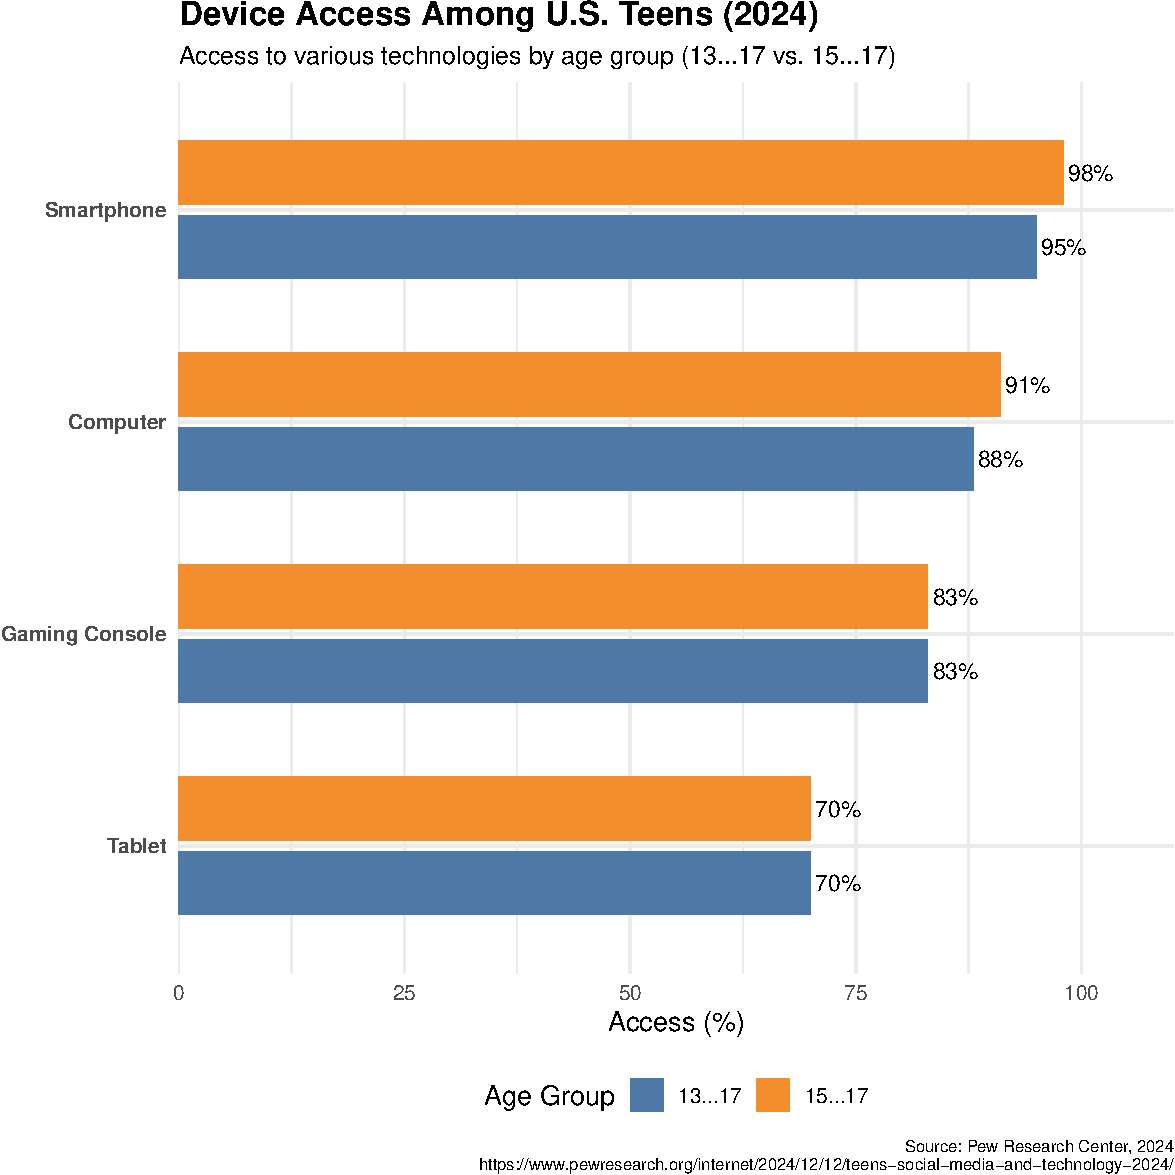
\includegraphics[keepaspectratio]{report_files/figure-pdf/smartphone-usage-1.pdf}}

\subsection{Used Terms and their
Definitions}\label{used-terms-and-their-definitions}




\end{document}
